\section{The \thelibos{} architecture}


The \libos{} of \graphene{}, or 
\thelibos{},
is a single library that resides beneath a Linux application,
for exporting compatible Linux features and API.
\thelibos{} guarantees reuse of an unmodified Linux application
upon \thehostabi{},
regardless of host limitations or distinctions.
%upon an incompatible host OS or hardware.
%to support compatible OS features.
%for exporting compatible features.
An unmodified Linux application assumes the existence of a Linux kernel or equivalent,
with idiosyncratic features and characteristics,
or so-called {\bf Linux personality}.
%which an unmodified Linux application depends on.
%In order to reuse an unmodified Linux application
%on an incompatible host,
\thelibos{} reproduces the Linux personality,
to act as a guest-level Linux kernel.
%over various host options.
%using \thehostabi{} exported by the host OS and PAL.
%The purpose of \thelibos{}
%is to resue an unmodified Linux application,
%by combining with a PAL and a host OS to behave as an equivalence of a Linux kernel. 
%%which is developed upon the assumption of running on a Linux kernel or equivalent.
%The main purpose of \thelibos{} is to reproduce
%the idiosyncratic features and behaviors of Linux,
%or the {\bf Linux personality},
%to resurrect Linux applications upon incompatible
%host OSes or hardware.
\graphene{} develops \thelibos{} as an ELF dynamic library (i.e., \code{\tt libLinux.so}),
and the PAL dynamically loads \thelibos{}.
%to be loaded on a host by the corresponding PAL.
%at the beginning of a \picoproc{}.


A key component of \thelibos{}
is a Linux system call table, which redirects \linuxapis{} from a Linux application.
%a key Linux kernel component applications. 
%that \thelibos{} implements is the Linux system call table.
%For Linux and similar OSes,
A system call table is an important entry point to a Linux kernel.
A system call table contains
pointers to the kernel functions that implements each \linuxapi{},
indexed by the \linuxapi{} numbers (e.g., \code{NR\_open}).
%and triggers in-kernel operations for servicing requests from applications.
%and defines the interaction between applications and kernel.
\graphene{} moves the Linux system call table into \thelibos{},
and develops \linuxapi{} handlers in the user space.
%The system call table in \thelibos{} contains a number of \linuxapi{} handlers,
Each \linuxapi{} handler emulates
the semantics of a \linuxapi{},
% that \graphene{} supports;
%\graphene{} develops each handler
based on either the specification % known by the Linux application developers,
described in the man pages~\cite{linux-man-syscall},
or the bug-for-bug behaviors
observed in a real Linux kernel.
Some \linuxapis{}, such as \syscall{rt\_sigaction}, are partially documented
in the man pages, and \thelibos{} imitates a Linux kernel on implementing a poorly-documented \linuxapis{}.
\graphene{} grows the \thelibos{} functionality
by extending the guest-level Linux system call table
with more complete implementation.

%Otherwise, for a few \linuxapis{} whose behaviors
%are not clearly defined by the Linux manpages,
%such as \syscall{rt\_sigaction},
%the \linuxapi{} handlers mimic the bug-for-bug behaviors of an actual Linux kernel.
%A continuing goal in \graphene{} is
%to extend \thelibos{} with more complete \linuxapi{} handlers.


%grow the functionality of \thelibos{},
%by extending the system call table with more complete handlers.




%The development of \linuxapi{} handlers in \thelibos{}
%is equivalent to implementing the specifications described in the Linux man pages~\cite{linux-man-syscall},
%including the valid inputs to each \linuxapi{},
%as well as the expected outcome.


%\paragraph{Implementing Linux Personality.} 
%\fixmedp{Revisit the logical flow of these paragraphs}
\Thelibos{} currently implements \graphenesyscallnum{} \linuxapis{},
and is sufficient to run a range of applications from servers to command-line programs or runtimes.
For reference, a recent Linux kernel supports more than 300 \linuxapis{}.
Among \~300 \linuxapis{}
there is a long tail of infrequently-used \linuxapis{}.
%upon \thehostabi{}. % to interact with the host.
%Among the whole Linux \linuxapi{} table,
%A Linux kernel exports a long tail of infrequently-used \linuxapis{}.
%For reference, the Linux \linuxversion{} kernel exports \linuxsyscallnum{} \linuxapis{}.
A study of the Linux \linuxapi{} usage~\cite{tsai16apistudy}
indicates that only 40 \linuxapis{} are indispensable to every applications released in the Ubuntu official repositories.
%The study also shows that
In the meantime, more than 100 \linuxapis{} are used by only exactly one application,
or none at all.
The development of \thelibos{} begins with
implementing 12 \linuxapis{}, such as \syscall{read} and \syscall{open}, which are fundamental to running a ``hello world'' application,
%such as \syscall{read}, \syscall{write}, and \syscall{open},
and gradually grows the \linuxapi{} count.
%for each new application introduced to run on \graphene{}.
%As the count of \linuxapis{} continues to grow,
Each time \thelibos{} is tested against a new application, the number of \linuxapis{} that need to be added has dropped.
%Based on the types of applications priorized in \graphene{}, including servers, command-line programs, and language runtimes, some \linuxapis{} to be more important %for reusing the applications
%than the others. % \linuxapis{}.
%According to the usage of each \linuxapi{} in applications,
\graphene{} prioritizes the popular \linuxapis{}, and leaves other \linuxapis{} that are either unpopular or for administrative purposes such as rebooting
or configuring network interfaces.
\thelibos{} demonstrates the sufficiency of
implementing Linux \linuxapis{} upon \thehostabi{},
for a representative subset of applications, .


%The current \thelibos{} implementation
%includes a set of high-valued Linux \linuxapis{} for the types of applications
%that \graphene{} has targeted,
%including servers, command-line programs, and runtimes.
%The remaning \linuxapis{} may require extending \thehostabi{} with more privileged abstractions,
%including administrative operations
%and host-specific features.
%\thelibos{} demonstrates that \thehostabi{} is sufficient
%for exporting the host abstractions, to support a representative sample of Linux applications.

%such as memory sharing, scheduler configuration, and NUMA (non-uniform memory architecture) support.


%Linux exports a very long tail of infrequently-used \linuxapis{}.
%applications.




%An analysis indicates roughly 100 additional calls that can be implemented
%with the existing \pal{} ABI and coordination framework, less than 10 administrative calls that will not make sense to expose to 
%an application, such as loading a kernel module or rebooting the system, and roughly 54 that will require 
%\pal{} extensions to meaningfully implement, such as controlling scheduling,
%NUMA placement, I/O privilege, and shared memory.
%In the last category of system calls, the degree to which actual host details should be exported versus emulated is debatable.

%We believe represent the most commonly used system calls.
%When an application requests a call or argument that {\tt libLinux.so} does not implement,
%the picoprocess exits with a distinct error message. 
%Each time we have tested \graphene{} with a new application, the number of extra system calls
%required has dropped---most recently we only added 4 calls
%(namely, epoll\_create, epoll\_wait, semget and semop)
%to support the Apache web server.
%Thus, we believe \graphene{} implements a representative sample of Linux calls.

%such as {\tt sched\_setparam}, which manipulates scheduler-specific
%parameters or 
%{\tt uselib}, which has been abandoned 
%in {\tt glibc} version 2 in favor of a user-space dynamic linker.
%We do not plan to implement administrative interfaces, such as {\tt reboot}.
%The growth in the set of supported system calls has been driven by 
%the requirements of new applications we use to exercise \graphene{}, and has been 
%slowing considerably over time.



\subsection{\Linuxapi{} redirection}
\label{sec:libos:syscall-redirection}


\thelibos{} transparently redirects \linuxapis{} from a Linux application. In a Linux kernel, a \linuxapi{} interrupt handler
triggers the kernel operations
whenever an application executes
a ``\assembly{syscall}'' or ``\assembly{int \$80}'' instruction.
The interrupt handler
switches the context of application,
and then jumps to the kernel routines which serve the \linuxapis{}.
%based on a kernel convention agreed by applications and Linux kernels.
Because \thelibos{} reuses
unmodified Linux executables and libraries,
it must redirect
unmodified \linuxapi{} invocation
to its
system call table. % implemented inside \thelibos{}.
%intercepts the \linuxapis{}
%in an executable or library binary, and redirect the \linuxapis{}
%to the \linuxapi{} handlers inside \thelibos{}.
%\thelibos{} implements the callback functions for a subset of the Linux \linuxapis{}.
%For reference, Linux kernel \linuxversion{}
%has defined \linuxsyscallnum{} \linuxapis{} in total.


Normally,
\thelibos{} redirects \linuxapis{} %from an unmodified Linux application
by modifying the C library (\libc{}).
%from an unmodified Linux application.
Most Linux executables and libraries
are linked against \libc{},
and rely \libc{} functions to access OS features
instead of
invoking \linuxapis{} directly.
%but use \libc{} functions as wrappers to \linuxapis{}.
%which internally execute ``\code{syscall}'' or ``\code{int \$80}'' instructions.
%an executable or library in Linux and similar OSes invokes \linuxapis{} through \libc{},
%instead of directly containing the \code{syscall} instructions.
%The \libc{}
%contains a large set of \linuxapi{} wrappers,
%which encapsulate direct \linuxapis{} to the kernel as functions.
For example,
compared with making the \syscall{read} \linuxapi{} directly,
more commonly
an application uses \libc{}'s \code{stdio} functions,
or calls the \libc{} \syscall{read} wrapper
%\funcname{read} is a wrapper to,
which internally runs \assembly{syscall}.
% that bares the same name and definition.
Unless configured otherwise, \thelibos{} uses a modified
{\bf GNU C library (\glibc{})}~\cite{glibc},
as the standard GNU \libc{} of most Linux distributions, including Ubuntu.
%applications released by Ubuntu. % are compatible against \glibc{}.
%which is compatible against most of the Linux applications released for Ubuntu.
%Other \libc{} variants, ,
%which are either fully or partially compatible with \glibc{},
%can be also modified to redirect \linuxapis{} to \thelibos{}.
%are alternatives upon \thelibos{} as long as they are modified for .
\graphene{} can be configured to use other \libc{} variants,
such as \projname{uClibc}~\cite{uclibc} and \projname{musl}~\cite{musl},
if an application finds them sufficient.
%\graphene{} demonstrates that 
%are also demonstrated
%to be acceptable alternatives,
%with slight modification for \linuxapi{} redirection.




\graphene{} modifies only \gipclines{} lines of the \glibc{} code.
The C source code in \glibc{} uses a platform-independent macro,
%referenced a single macro called
\funcname{INLINE\_SYSCALL},
to invoke \linuxapis{} to the kernel.
%when it needs to invoke a \linuxapi{}.
\funcname{INLINE\_SYSCALL} contains a piece of assembly code
that copies \linuxapi{} number and arguments to registers,
and then uses \assembly{syscall} to enter a Linux kernel.
\graphene{} modifies \funcname{INLINE\_SYSCALL}
to redirect a \linuxapi{} to
an entry point of \thelibos{} called \funcname{syscalldb}.
\funcname{syscalldb} saves the current register state, similar to a context switch,
and then
calls the \linuxapi{} handler
indicated by the \linuxapi{} number.
%, to trigger operations inside \thelibos{}.
For assembly code in \glibc{},
\graphene{} replaces each \code{syscall} instruction with
a dynamic call to
\funcname{syscalldb}, given the address of \funcname{syscalldb} is dynamically determined.
Figure~\ref{fig:libos:syscall-redirection} summarizes the mechanism of \linuxapi{} redirection.
%to \thelibos{}.


\begin{figure}[t!]
\centering
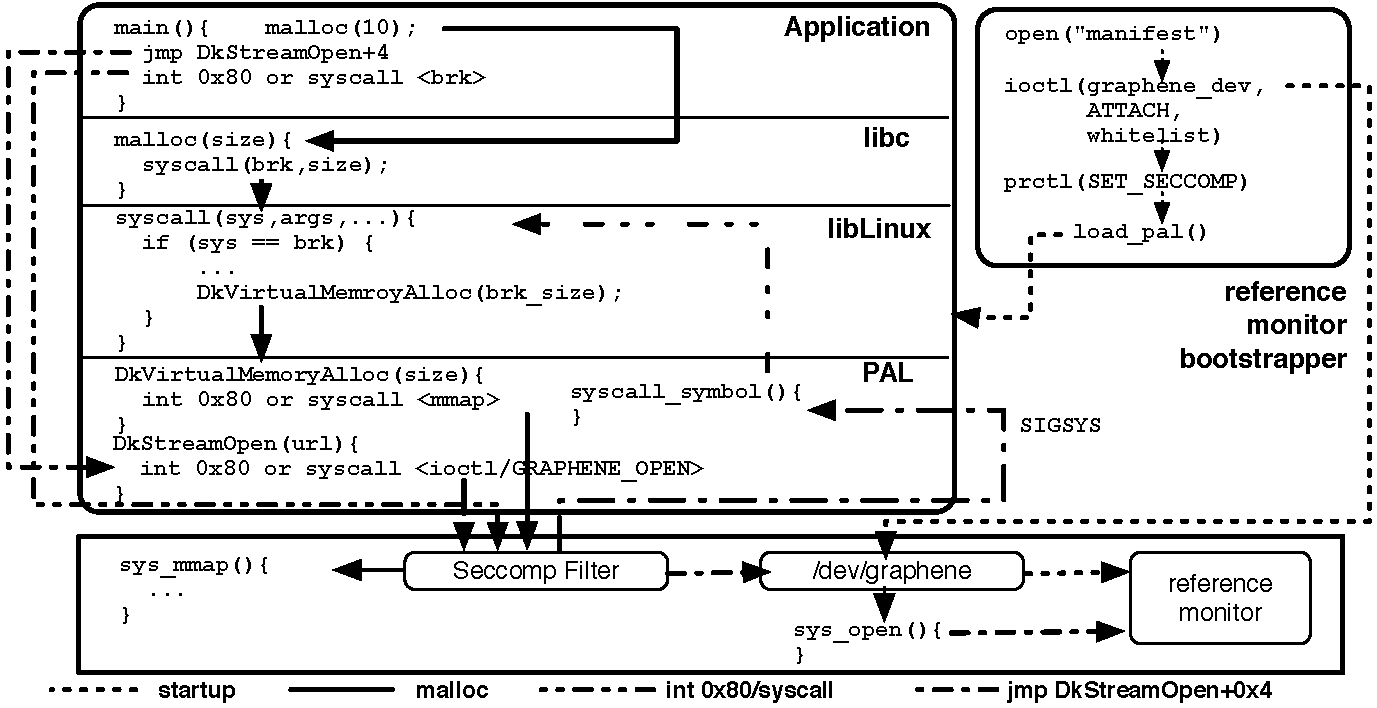
\includegraphics[width=32em]{syscall-redirection.pdf}
\footnotesize
\caption{System call redirection for \thelibos{}.
In the normal case (the first instruction of \funcname{main}), \funcname{malloc} internally invokes 
\syscall{mmap}, which is redirected to \funcname{syscalldb} in \thelibos{}.\thelibos{} then invokes a \hostapi{}, \palcall{VirtMemAlloc}, to allocate host memory. The second instruction of \funcname{main} invokes a direct \linuxapi{}, which is trapped by the host-level exception handler,
and returned to \funcname{IllegalInstrHandler} in \thelibos{}.}
\label{fig:libos:syscall-redirection}
\end{figure}


\graphene{} modifies four \glibc{} libraries:
%When using \graphene{}, an application must be deployed with the modified \libc{} libraries,
the runtime loader (\code{ld.so}), the core library (\code{libc.so}), the pthread library (\libpthread{}), and the dynamic loading library (\libdl{}).
Each of the \Glibc{} libraries has separate purposes and features,
and is mostly loaded on demand except \code{ld.so}.
%Despite that \glibc{} has partitioned its code into separate libraries,
\graphene{} only modifies the \glibc{} libraries which contains direct \assembly{syscall} instructions.
%not every libraries of \glibc{} need to be modified for \linuxapi{} redirection.
%Only \code{libc.so}, \libpthread{}, and \libdl{} have included \code{syscall} instructions,
%and thus have to be modified for \graphene{}.
Other libraries, such as \code{libm.so},
only rely on 
existing \libc{} functions,
so \graphene{} leaves these libraries unmodified.



\paragraph{Hard-coded \linuxapis{}.}
Static binaries, or some platform-dependent applications, contain hard-coded \assembly{syscall} instructions
which cannot be redirected by a modified \libc{}.
Application developers
create a static binary with with hard-coded \linuxapis{} by statically linking a local version of \libc{} as part of the binary.
%as a static binary with hard-coded \linuxapis{}. %\code{syscall} instructions.
It is also possible to program an application
with assembly code that directly invokes \linuxapis{}---usually in a language runtime (e.g., the go runtime) or a system software (e.g., \projname{busybox}).
%---with assembly code that directly invokes
%platform-depenedent,
%rare \linuxapis{} that are not wrapped by \libc{} functions.
%one of the \linuxapi{} wrappers in \libc{}, or \funcname{syscall}.
%As a result, a ELF binary may contain hard-coded \assembly{syscall} instructions.
%Either way leads to hard-coding \code{syscall} instructions in the ELF binaries.
Because a modified \libc{} cannot redirect hard-coded \linuxapis{},
the application switches context into the host kernel,
causing security and compatibility breaches by exposing unauthorized or unsynchronized host OS states to the application.



\thelibos{} needs support from a host OS to restrict direct \linuxapis{} from an application.
%\thelibos{} depends on host-level \linuxapi{} restriction to redirect hard-coded \linuxapis{}.
%to prevent \linuxapis{} from anywhere other than a PAL.
A Linux kernel allows an application to install a \linuxapi{} filter in the Berkeley Packet Filter (BPF) format,
called a \seccomp{} filter~\cite{seccomp}.
A \seccomp{} filter can block or forward a \linuxapi{} based on the \linuxapi{} number,
argument values, or the code address that invokes the \linuxapi{}.
%A direct \linuxapi{} traps into the host kernel,
%unless the host has virtualized the interrupt handler to the \libos{}.
\graphene{} relies on the hosts to install a \linuxapi{} filter, or enforce architectural restriction, to detect direct \linuxapis{}.
For example, SGX already has a restriction that an enclave application cannot trigger any \linuxapi{} to switch context into the untrusted kernel.
% inside an enclave and triggers an exception for an in-enclave \linuxapi{}.
%\code{syscall} instructions
%(e.g., SGX restriction).
%The details of the \linuxapi{} restriction mechanisms are discussed in
%\fixme{update labels}
%Section~\ref{sec:linux:syscall} and Section~\ref{sec:sgx:syscall}.
If the host detects a direct \linuxapi{} from an application,
it can return
a PAL exception to an exception handlers assigned by \thelibos{}, using  \palcall{ExceptionSetHandler}.
%\thehostabi{} specifies that the host captures unauthorizes \linuxapis{}
%and redirects to an exception handler (set up by \palcall{ExceptionSetHandler}).
%If a binary makes an illegal \linuxapi{},
%the host-level \linuxapi{} restriction will trigger an \code{ILLEGAL} exception
%at \thehostabi{},
%and thus the \linuxapi{} is redirected by an exception handler
%assigned by \thelibos{}.
The exception handler can recover the \linuxapi{} number and arguments
from the context saved at the \linuxapi{},
and forward the \linuxapi{} to the \linuxapi{} handler
inside \thelibos{}.


Using exceptions to forward direct \linuxapi{} is much slower than redirecting through a modified \libc{},
due to the overhead of switching context between the application and the host kernel.
To handle an exception from the host OS,
the application at least switches context twice, including both triggering the exception handler and returning to the original execution.
To mitigate the overhead,
\thelibos{} can 
rewrite the hard-coded \assembly{syscall} or \assembly{int \$80} inside each application binary during the run time.
% to redirect the hard-coded \linuxapis{};
%use {\bf binary translation} to modify the hard-coded \code{syscall} instructions;
There can be two timings for rewriting the instructions:
One is the timing when the runtime loader a new binary, and \thelibos{} can perform a full scan of the binary
to replace \assembly{syscall} or \assembly{int \$80} with a jump to \thelibos{}'s \linuxapi{} table.
\thelibos{} can also passively replace the instructions
whenever the host detects a direct \linuxapi{} and triggers an exception handler.
%binary translation
%can be triggered when a host-level exception is raised
%for an illegal \linuxapi{},
%to optimize consecutive \linuxapi{} invocation at the same location.
%\thelibos{} can also perform a full scan in application binaries
%to spot and modify hard-code \code{syscall} instructions.
\graphene{} leaves binary rewriting
as a future feature.


